% Opcje klasy 'iithesis' opisane sa w komentarzach w pliku klasy. Za ich pomoca
% ustawia sie przede wszystkim jezyk i rodzaj (lic/inz/mgr) pracy, oraz czy na
% drugiej stronie pracy ma byc skladany wzor oswiadczenia o autorskim wykonaniu.\\
%\ifx\HCode\UnDef\else\hypersetup{tex4ht}\fi
\documentclass[declaration,shortabstract]{iithesis}
\usepackage{polski}
\usepackage[utf8]{inputenc}
\usepackage{listings}
\usepackage{float, graphicx}
\usepackage[backend=bibtex,style=verbose-trad2]{biblatex}


%%%%% DANE DO STRONY TYTYŁOWEJ
% Niezaleznie od jezyka pracy wybranego w opcjach klasy, tytul i streszczenie
% pracy nalezy podac zarowno w jezyku polskim, jak i angielskim.
% Pamietaj o madrym (zgodnym z logicznym rozbiorem zdania oraz estetyka) recznym
% zlamaniu wierszy w temacie pracy, zwlaszcza tego w jezyku pracy. Uzyj do tego
% polecenia \fmlinebreak.
\polishtitle    {Analiza drzew samoorganizujących}
\englishtitle   {Analysis of self adjusting binary search trees}
\polishabstract {Binarne drzewa wyszukiwań (BST) to jedna z najbardziej podstawowych struktur danych w informatyce. Struktura ta jest reprezentacją zbioru elementów i umożliwia wyszukiwanie elementów. Dla konkretnego ciągu zapytań można znaleźć optymalne drzewo BST, które zrealizuje go w minimalnym czasie. Wymaga to jednak znajomości całego ciągu zapytań przy tworzeniu struktury, przez co nie jest to praktyczne rozwiązanie. Binarne drzewa wyszukiwań mają bardzo wiele zastosowań w informatyce. Z tego powodu powstało wiele algorytmów reorganizacji tej struktury danych, umożliających efektywne wykonywanie operacji wyszukiwania bez znajomości wszystkich zapytań. Możemy wyróżnić dwa rodzaje takich algorytmów: algorytmy balansujące ograniczające pesymistyczny czas wyszukiwania (przykładami są drzewa AVL, AA oraz czerwono-czarne) oraz algorytmy samoorganizujące wykorzystujące wiedzę o obsłużonych zapytaniach do przyspieszenia obsługi następnych zapytań. W tej pracy zaimplementuję oraz zbadam efektywność wybranych algorytmów samoorganizujących. Porównam czasy działania samoorganizujących algorytmów Tango i Splay z własną implementacją drzewa czerwono-czarnego, implementacją drzewa czerwono-czarnego ze standardowej biblioteki C++, oraz z optymalnym drzewem.}

\englishabstract{Binary search trees (BST) are one of the most elementary data structures in computer science. The data structure is a representation of a set of elements and supports lookup of particular element. For a defined sequence of queries it is possible to create an optimal BST, that answers the queries in minimal time. It requires, however, prior knowledge of the entire query sequence, which makes this solution impractical. Binary search trees have a multidute of applications in computer science. This prompted the invention of several algorithms for reorganising this data structure, and enabling the structure to handle queries more efficiently, without knowing the entire sequence of queries. We can destinguish two kinds of these algorithms : balancing algorithms,which limit the pessimistic of query processing (such as AVL, AA and black-red trees) and self adjusting algorithms, which use already the knowledge of already processed queries to speed up the processing of the coming queries. In this paper I will implement and test the efficiency of selected self adjusting algorithms. I will compare the runtimes of self adjusting Tang and Splay algorithms and compare them to my implementation of black-red tree, the C++ standard template library implementation of black-red tree and the optimal binary search tree}
% w pracach wielu autorow nazwiska mozna oddzielic poleceniem \and
\author         {Julia Majkowska}
% w przypadku kilku promotorow, lub koniecznosci podania ich afiliacji, linie
% w ponizszym poleceniu mozna zlamac poleceniem \fmlinebreak
\advisor        {dr hab. Marcin Bieńkowski}
%\date          {}                     % Data zlozenia pracy
% Dane do oswiadczenia o autorskim wykonaniu
\transcriptnum {290363}                     % Numer indeksu
%\advisorgen    {dr. Jana Kowalskiego} % Nazwisko promotora w dopelniaczu
%%%%%

%%%%% WLASNE DODATKOWE PAKIETY
%
%\usepackage{graphicx,listings,amsmath,amssymb,amsthm,amsfonts,tikz}
\usepackage{amsthm, amsmath}
%
%%%%% WŁASNE DEFINICJE I POLECENIA
%

\newcounter{thm}[section]
\renewcommand{\thethm}{\thechapter\arabic{thm}}
\def\claim#1{\par\medskip\noindent\refstepcounter{thm}\hbox{\bf \arabic{chapter}\arabic{thm} #1.}
\it\ %\ignorespaces
}
\def\endclaim{
\par\medskip}
\newenvironment{thm}{\claim}{\endclaim}
\theoremstyle{thm} 
\newtheorem{definition}[thm]{Definicja}
%\numberwithin{definition}{subsection}
\theoremstyle{remark} 
\newtheorem{remark}[thm]{Obserwacja}
%\numberwithin{remark}{subsection}
\theoremstyle{plain} 
\newtheorem{theorem}[thm]{Twierdzenie}
%\numberwithin{theorem}{subsection}
\theoremstyle{plain} 
\newtheorem{hypothesis}[thm]{Hipoteza}
%\numberwithin{hypothesis}{subsection}
\theoremstyle{plain} 
\newtheorem{lemma}[thm]{Lemat}
%\numberwithin{lemma}{subsection}
%\renewcommand \qedsymbol {\ensuremath{\square}}
% ...
%%%%%

\begin{document}

%%%%% POCZĄTEK ZASADNICZEGO TEKSTU PRACY

  

\chapter{Wprowadzenie}   

\section{Wstęp}   

Binarne drzewo przeszukiwań (inaczej BST) to jedna z najbardziej podstawowych struktur danych w informatyce. Stosuje się je w wielu systemach informatycznych i algorytmach. Ideą struktury jest trzymanie elementów w wierzchołkach, zawierających wartość elementu oraz wskaźniki na lewe i prawe poddrzewo. Elementy umieszcza się w strukturze w taki sposób, aby wszystkie wartości elementów znajdujące się w lewym poddrzewie wierzchołka \(w\) były elementami mniejszymi od \(w\) w zdefiniowanym porządku. Analogicznie wszystkie elementy w prawym poddrzewie są elementy większe w tym porządku. Na tak uporządkowanych danych można wyszukiwać daną wartość \(v\) poprzez zagłębianie się w drzewo wybierając odpowiednio lewe lub prawe poddrzewo w zależności od wyniku porównania \(v\) z wartością korzenia poddrzewa. W najbardziej podstawowej formie tej struktury operacje wstawiania, wyszukiwania i usuwania wykonuje się w czasie \(O(H)\), gdzie H to wysokość drzewa. W pesymistycznym wypadku jest to czas liniowy od liczby elementów w strukturze. Złożoność operacji słownikowych na drzewie BST zależy od głębokości drzewa, dlatego powstało wiele struktur danych ograniczających maksymalną głębokość drzewa. Spośród deterministycznych można wymienić drzewa Splay, AA, AVL oraz czerwono-czarne, obsługujące operacje słownikowe w pesymistycznym czasie \(O(\log n)\).   

 

\section{Problem optymalnego drzewa binarnego}   

W wielu zastosowaniach dane nie podlegają rozkładowi jednostajnemu tylko przejawiają jakąś lokalność. Przykładowo, jeśli dla drzewa 100-elementowego będą się pojawiać głównie zapytania o jeden element, można by znacząco zmniejszyć czas działania przesuwając dany element do korzenia. W takim wypadku struktura naszego drzewa zależy od zapytań. Problem znajdowania drzewa binarnego, które przy użyciu najmniejszej liczby operacji obsłuży ciąg zapytań to problem optymalnego drzewa binarnego. Możemy rozróżnić dwa warianty tego problemu: statyczny oraz dynamiczny.   

\subsection{Statyczne optymalne drzewo binarne}   

Wg. definicji Knutha w problemie statyczne optymalności binarnego drzewa wyszukiwań definiujemy uporządkowany ciąg elementów \(e_1...e_n\), ciąg prawdopodobieństw \(A_1...A_n\), będące prawdopodobieństwem wykonania wyszukiwania \(e_i\) i  \(B_0 … B_n\), będące prawdopodobieństwem wyszukania elementu z przedziału \([e_i, e_{i+1}]\). Szukamy drzewa minimalizujący oczekiwany czas wyszukiwania.   

Wraz z definicją problemu Knuth opublikował algorytm opierający się na programowaniu dynamicznym, znajdujący optymalne drzewo binarne w czasie O(\(n^2\)). W 1975 r. Mehlhorn opublikował algorytm aproksymujący ten problem, działający w czasie \(O(n)\). Dla wariantu, w którym \(B_i = 0\), istnieje algorytm Garsia-Wachsa, który znajduje optymalne drzewo w czasie \(O(n\log n)\).   

\subsection{Dynamiczne optymalne drzewo binarne}   

W dynamicznym wariancie problemu mamy na wejściu ciąg zapytań \(X  = \{x_1,x_2,..., x_n\}\) o wyszukanie klucza \(x_i \in {1, 2, ..., n}\). Dla każdego zapytania o wartość \(w\) zaczynamy ze wskaźnikiem na korzeń drzewa i wykonując tylko niżej wymienione operacje chcemy przesunąć wskaźnik na wierzchołek zawierający klucz o wartości \(w\). Dozwolone operacje to:   

\begin{enumerate}   

\item {Przesunąć wskaźnik na lewego syna obecnie wskazanego wierzchołka}   

\item {Przesunąć wskaźnik na prawego syna obecnie wskazanego wierzchołka}   

\item {Przesunąć wskaźnik na rodzica obecnie wskazanego wierzchołka}   

\item {Wykonać pojedynczą rotację obecnie wskazywanego wierzchołka. Poniżej ilustracja pojedynczej rotacji punku p w prawo}    

\end{enumerate}   
\begin{figure}[H]
\centering    
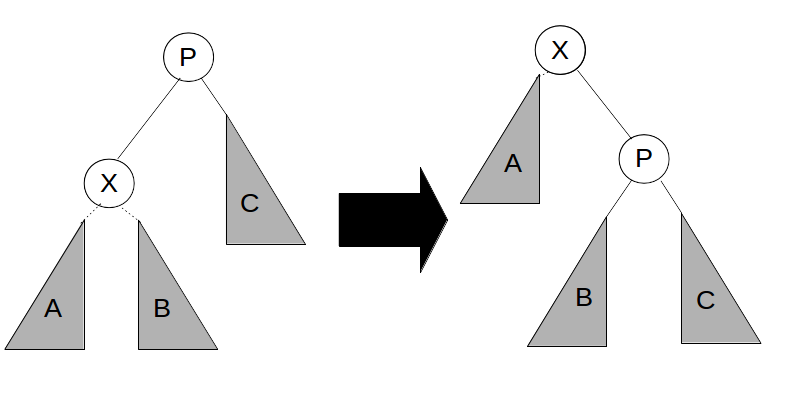
\includegraphics[scale = 0.5]{zig.png}  
\caption{Pojedyncza rotacja w prawo w punkcie p} 
 \label{fig:1} 
\end{figure}  

 
W tym problemie chcemy znaleźć drzewo, które minimalizuje liczbę operacji koniecznych do obsłużenia ciągu zapytań \(x_i\). 

\begin{definition}[Konkurencyjność]
Oznaczmy wejscie dla algorytmu jako \(\sigma\), koszt algorytmu dla tego wejścia jako \(ALG(\sigma)\) i optymalny koszt jako \(OPT(\sigma)\).
Mówimy, że algorytm jest $k$ konkurencyjny, jeśli
\begin{align*}
\forall_{\sigma} ALG(\sigma) \leq k*OPT(\sigma)
\end{align*}
Liczbę $k$ będziemy nazywali współczynnikiem konkurencyjności.
\end{definition}  

Dla każdego ciągu zapytań istnieje minimalny ciąg operacji odpowiadający na te zapytania. Znalezienie takiego rozwiązania wymaga znajomości całego ciągu zapytań z góry, co w wielu sytuacjach nie jest możliwe. Będziemy mówić, że drzewo jest dynamicznie optymalne ma stały współczynnik konkurencyjności. Udowodnienie dynamicznej optymalności dowolnego algorytmu BST jest problemem otwartym.   

\chapter{Statyczne drzewo optymalne}

\section{Opis struktury}

Oznaczmy ciąg zapytań jako \( X = \{x_1, x_2, ..., x_m\}\), i zbiór elementów, które występują w tym ciągu jako \( Y = \{y_1, y_2, ..., n\}\), gdzie \(y_{i-1} < y_i < y_{i+1}\). 
Dodatkowo niech \(C(y)\) będzie liczbą wystąpień \(y\) w ciągu \(X\). 
Przyjmijmy, że nasze klucze \(y_i\) umieszczamy na jakimś drzewie BST, dla danego drzewa BST \(\mathcal{B}\) i elementu \(y_i\) \( d(\mathcal{B}, y_i)\) to głębokość wierzchołka zawierającego \(y_i\) w \(\mathcal{B}\). 
Zdefiniujmy sobie koszt obsługi zapytania na drzewie \(\mathcal{B}\) jako \(K(x_i) = d(\mathcal{B}, x_i)\).
Statyczne drzewo optymalne to takie drzewo, które dla danego ciągu zapytań, obsługuje je minimalnym sumarycznym kosztem. 
Na tym drzewie nie wkonujemy żadnych rotacji, a jego struktura pozostaje stała, przez cały czas obsługi zapytań. 
Ze względu na swój statyczny charakter drzewo to obsługuje jedynie operację wyszukiwania na drzewie.

\section{Algorytm konstrukcji drzewa}

Statyczne drzewo optymalne można skonstruuować przy pomocy programowania dynamicznego. Wprowadźmy sobie następujące oznaczenia, niech \(Cost(i, j)\) będzie oznaczał minimalny koszt obsłużenia \(\{ x : x\in X \wedge x\in \{y_i, y_{i+1}, ..., y_{j}\}\}\) optymalnym drzewem BST składającym się z elementów \(\{y_i, y_{i+1}, ..., y_{j}\}\) , a \(Root(i, j)\) niech będze indeksem korzenia tego optymalnego drzewa. Dodatkowo niech \(Sum(i, j) = \sum_{k = i}^j C(y_k)\).

Zacznijmy od zdefiniowania przypadków bazowych: 
\begin{align*}
Cost(i, i) = C(y_i)\\
Root[i][i] = i
\end{align*}
Zauważmy, że jeśli \(Root(i, j) = r\) wtedy \(Cost(i, j) =  Cost(i, r-1) + Cost(r+1, j) + Sum(i, j)\). W takim razie możemy zapisać następujące zależności rekurencyjne:
\begin{align*}
Root(i, j) = argmin_r Cost(i, r-1) + Cost(r+1, j) + Sum(i, j)\\
Cost(i, j) =  Cost(i, Root(i, j)-1) + Cost(Root(i, j)+1, j) + Sum(i, j)\\
\end{align*}

W ten sposób otrzymujemy algorytm tworzenia drzewa o złożoności \(O(n^3)\). 

\begin{theorem}[Knuth, 1971]
\label{root_constr}
\(Root(i, j-1) \leq Root(i, j) \leq Root(i+1, j)\)
\end{theorem}

\begin{remark}
Korzystając z \ref{root_constr} możemy ograniczyć koszt działania tworzenia optymalnego drzewa BST do \( 0(n^2)\)
\end{remark}
\begin{proof}
Policzmy sumarycznyczny koszt działania algorytmu.
\begin{align*}
&\sum_{i=1}^n \sum_{j = i}^n Root(i+1, j) - Root(i, j-1) + 1 \\
&\leq  n^2 + \sum_{i=1}^n \sum_{j = 1}^n Root(i+1, j) - \sum_{i=1}^n \sum_{j = 1}^n Root(i, j -1) \\
&= n^2 + \sum_{i=2}^{n+1} \sum_{j = 1}^n Root(i, j) - \sum_{i=1}^n \sum_{j = 0}^{n-1} Root(i, j) \\
&\leq n^2 + \sum_{i=1}^{n+1} \sum_{j = 1}^n Root(i, j) - \sum_{i=1}^n \sum_{j = 1}^{n-1} Root(i, j) \\
&= n^2 + ( \sum_{i=1}^{n} \sum_{j = 1}^n Root(i, j) - \sum_{j=1}^n Root(n+1, j) ) - ( \sum_{i=1}^{n} \sum_{j = 1}^n Root(i, j) - \sum_{i=1}^n Root(i, n) )\\
&= n^2 + \sum_{i=1}^n Root(i, n) - \sum_{j=1}^n Root(n+1, j)\\
&= O(n^2)
\end{align*}
\end{proof}

\section{Opis implementacji}

Implementacja statycznego drzewa optymalnego składa się z dwóch klas \texttt{static\_tree} i \texttt{tree\_vert}. Klasa \texttt{tree\_vert} zostanie opisana w kolejnym rozdziale. 
\subsection{static\_tree}
Klasa \texttt{static\_tree<T>} udostępnia następujące metody:
\begin{itemize}
\item{ Konstruktor \texttt{static\_tree(const vector<int>\&)} - konstruuje drzewo korzystając z listy zapytań do obsłużenia. Zakłada się, że wyszystkie elementy z zapytań występują w strukturze}
\item{ \texttt{bool find(T)} - wykonuje wyszukiwanie na optymalnym drzewie binarnym i zwraca czy element znajduje się w strukturze}
\item{ Destruktor niszczący całą strukturę}
\end{itemize}
Z racji, że struktura ta jest statyczna operacje wstawiania oraz usuwania elementów nie są obsługiwane. 

\chapter{Drzewa Splay}   

\section{Opis struktury}  

Drzewo Splay zostało stworzone w 1985 przez Sleatora i Trajana \cite{DBLP:journals/jacm/SleatorT85}.

Drzewo Splay jest drzewem samoorganizującym się. Podstawą działania tej struktury jest operacja splay, polegająca na przesunięciu odpowiedniego wierzchołka do korzenia, korzystając z rotacji.   

\subsection{Splay}  

Operacja splay dla danego wierzchołka odbywa się w krokach, do momentu, kiedy wierzchołek nie stanie się korzeniem. Możemy wyróżnić 3 przypadki kroków operacji splay: \begin{enumerate}  

\item{ZIG - Jeśli $x$ jest lewym synem korzenia wykonujemy pojedynczą rotację korzenia w prawo. Analogicznie kiedy $x$ jest prawym synem korzenia wykonujemy rotację korzenia w lewo.\\  
\begin{figure}[H]
\centering
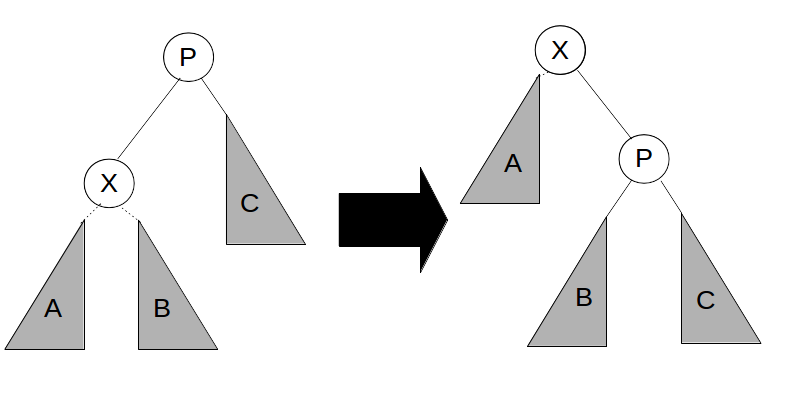
\includegraphics[scale = 0.3]{zig.png}  
\caption{Krok ZIG operacji Splay}  
\label{fig:zig} 
\end{figure}}   

\item{ZIGZIG - Jeśli zarówno $x$ i jego ojciec są lewymi synami wykonujemy u dziadka rotację w prawo, a następnie rotujemy w prawo ojca $x$. Analogicznie postępujemy kiedy $x$ i jego ojciec są prawymi synami.\\  

\begin{figure}[H]  
\centering
    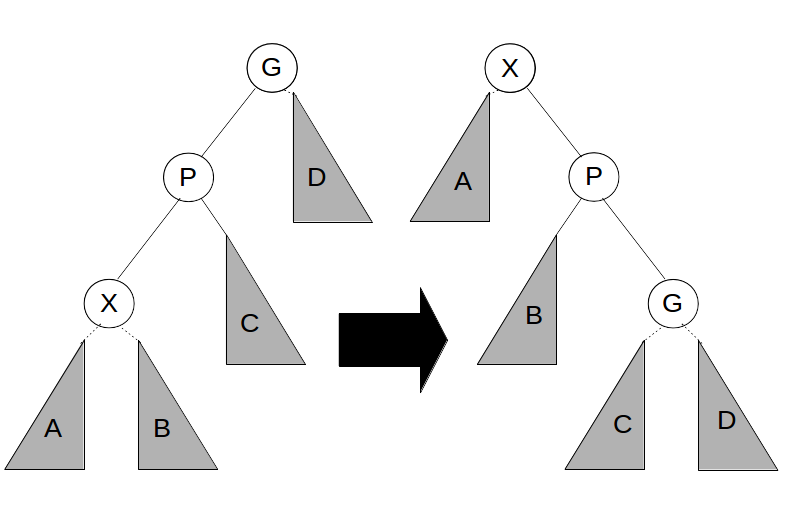
\includegraphics[scale = 0.3]{zigzig.png}
      \caption{Krok ZIGZIG operacji Splay}  
      \label{fig:zigzig} 
      \end{figure}}  

\item{ZIGZAG - Jeśli $x$ jest prawym synem, a jego ojciec jest lewym synem, rotujemy ojca $x$ w lewo a następnie dziadka $x$ (nowego ojca $x$) w prawo. Analogicznie postępujemy kiedy $x$  jest lewym synem, a jego ojciec jest lewym synem.\\ 
\begin{figure}[H] 
\centering    
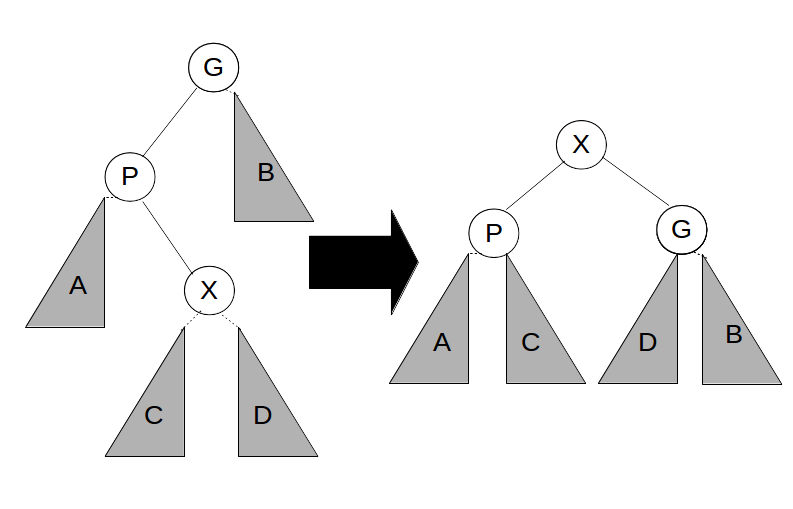
\includegraphics[scale = 0.3]{zigzag.png}  
\caption{Krok ZIGZAG operacji Splay}  
\label{fig:zigzag} 
\end{figure}} 
\end{enumerate}    

\subsection{Wyszukiwanie}
Drzewo splay spełnia zależność BST, więc można wyszukiwać w nim elementy jak w normalnym drzewnie BST. Po znalezieniu odpowiedniego wierzchołka wykonujemy na nim operację splay przenosząc go do korzenia.  

\subsection{Rozdzielanie drzewa względem elementu} 
Aby rozdzielić drzewo względem danego elementu, wyszukujemy go w drzewie i wykonujemy operację splay na elemencie, na którym zakończyliśmy poszukiwanie. Wynikiem będą lewe i prawe poddrzewo korzenia zmodyfikowanego drzewa.  

\subsection{Łączenie dwóch drzew} 
Będziemy łączyć drzewa \(d_1\) i \( d_2\) o własności, że \(\forall_{k_1 \in d_1, k_2 \in d_2} k_1 < k_2\). Aby to zrobić wykonujemy operację splay na wierzchołku zawierającym minimalny element \(d_2\). Następnie podłączamy \(d_1\) jako lewe poddrzewo zmodyfikowanego \(d_2\).  

\subsection{Wstawianie} 
Aby wstawić element \(e\) do drzewa najpierw wyszukujemy go w drzewie, jeśli element już znajduje się w drzewie to wykonujemy operację splay na odpowiadającym mu wierzchołku. Jeśli elementu nie ma w drzewie, wtedy rozdzielamy drzewo względem \(e\) na drzewa \(d_1\) i \( d_2\). Następnie podłączamy \(d_1\) jako lewe poddrzewo elementu  \(e\), a \(d_2\) jako prawe poddrzewo.  

\subsection{Usuwanie} 
Aby usunąć element, wyszukujemy go w drzewie i wykonujemy na odpowiadającym wierzchołku operację splay. Następnie łączymy lewe i prawe poddrzewo w jedną strukturę.  

\section{Analiza złożoności}  

\subsection{Złożoność pamięciowa} 
W każdym węźle trzymamy dwa wskaźniki na synów oraz wartość klucza. Cała struktura zajmuje pamięć $ O(n)$.  

\subsection{Analiza zamortyzowana złożoności czasowej} 
\begin{theorem} 
Dla ciągu zapytań $X = \{ x_1, x_2, ..., x_m\}$, gdzie \( \forall_{1\leq i \leq m} x_i \in \{1, 2,...,n\}\), drzewo splay działa w czasie \( O((m+n)logn)\). 
\end{theorem} 
\begin{proof} Zauważmy, że główną składową kosztu operacji słownikowych jest operacja splay. Pozostałe części operacji można wykonać w czasie stałym. Przeprowadzimy analizę zamortyzowaną kosztu wykonywania operacji splay. Wprowadźmy następujące oznaczenia : 
\begin{itemize} 
\item{\(s(w)\) - liczba wierzchołków w poddrzewie wierzchołka \(w\)} 
\item{\(r(w) = \lfloor log(s(w)) \rfloor\)} 
\item{Funkcja potencjału \(\Phi = \sum_w r(w)\)} 
\end{itemize}  

Przeanalizujmy najpierw zmianę potencjału \(\Phi\) przy poszczególnych krokach operacji Splay. Będziemy korzystali z notacji na schematach \ref{fig:zig}, \ref{fig:zigzig}, \ref{fig:zigzag} \\ 
\begin{enumerate} 
\item{\textbf{ZIG} : Zmienia się tylko potencjał $x$ i $p$
\begin{align*} 
\Delta \Phi & = 1 + \Delta r(x) + \Delta r(p) \\
 & = 1 + r'(x) - r(x) + r'(p) - r(p) \\ 
 & = 1 + r'(p) - r(x) && \text{ ponieważ }r'(x) = r(p)\\ 
 \end{align*}} 
\item{\textbf{ZIGZIG} : Zmienia się potencjał $x$, $p$ i $g$ 
\begin{align*} 
\Delta \Phi & = 2 + r'(x) - r(x) + r'(p) - r(p) + r'(g) - r(g)\\ 
& =2 - r(x) + r'(p) - r(p) + r(g)   && \text{ ponieważ } r'(x) = r(g)\\ 
& \leq 2 + r'(g) + r'(x) - 2r(x) && \text{ ponieważ } r(x) < r(p) \text{ i } r'(x) > r(p)\\ 
& \leq 3(r'(x) - r(x)) && \text{ z wypukłości funkcji logarytmicznej}\\ 
\end{align*}} 
\item{\textbf{ZIGZAG} : Zmienia się potencjał $x$, $p$ i $g$ 
\begin{align*} 
\Delta \Phi & =  2 + r'(x) - r(x) + r'(p) - r(p) + r'(g) - r(g)\\ 
& = 2 - r(x) + r'(p) - r(p) + r(g)   && \text{ ponieważ } r'(x) = r(g)\\ 
& \leq 2 + r'(g) + r'(p) - 2r(x) && \text{ ponieważ }r(x) < r(p)\\ 
& \leq 2(r'(x) -2r(x)) && \text{ ponieważ } 2r'(x) - r'(p) - r'(g) \geq 2\\ 
\end{align*}} 
\end{enumerate} 
We wszystkich przypadkach koszt operacji jest zatem nie większy niż \( 3(r'(x) - r(x)) + 1\), gdzie czynnik 1 występuje tylko przy operacji ZIG, a zatem tylko raz przy każdej operacji Splay. Dla całej operacji Splay(\(x_i\)) musimy zsumować zmianę potencjału wszytkich kroków. Otrzymujemy w ten sposób sumę teleskopową skracającą się do \(3(r(\text{korzeń}) - r(x_i)) + 1 \leq logn\). Aby otrzymać oszacowanie całego czasu działania na całej sekwencji $X$, musimy jeszcze uwzględnić zmianę potencjału pomiędzy stanem początkowym a końcowym : \( \sum_x r'(x) - r(x) \leq \sum_x O(logn) = O(nlogn)\). Zatem sumaryczny czas działania to \( O((m+n)logn)\).  

\end{proof}  

\section{Konkurencyjność} 
\begin{hypothesis} 
Drzewo splay jest dynamicznie optymalne tzn. \(SPLAY(X) = O(OPT(X)\) gdzie \(SPLAY(X)\) to koszt obsłużenia ciągu zapytań \(X\) przez drzewo splay, a \(OPT(X)\) przez optymalne dynamiczne drzewo działające offline. 
\end{hypothesis}  

\section{Opis implementacji}  

Implementacja składa się z dwóch klas \texttt{splay\_tree} i \texttt{tree\_vert}. 

\subsection{tree\_vert}

Ta klasa reprezentuje wierzchołek drzewa binarnego oraz jego poddrzewo. Udostępnia następujące metody: 

\begin{itemize}

\item{Konstruktory \texttt{tree\_vert(T val, tree\_vert<T>*f = NULL, tree\_vert<T>*l = NULL, tree\_vert<T>*r = NULL, bool is\_null = false)} tworzący wierzchołek trzymający wartość. Umożliwia ustawienie ojca wierzchołka (f), lewego syna (l), prawego syna (r) oraz wartość oznaczającą czy wartość w wierzchołku ma być traktowana jako cześć drzewa (is\_null)}
\item{Konstruktor \texttt{tree\_vert()} tworzący pusty wierzchołek którego wartość nie jest częścią drzewa}

\item{Desktruktor zwalniający wszystkie wskaźniki w poddrzewie}

\item{\texttt{void disown\_left()} i \texttt{void disown\_right()} - obcinają odpowiednio lewego i prawego syna wierzchołka.}
    
\item{\texttt{bool hook\_up\_left(tree\_vert<T>*)} i \texttt{bool hook\_up\_right(tree\_vert<T>*)} - podpinają wierzchołek z argumentu jako odpowiednio lewego i prawego syna wierzchołka.}

\item{\texttt{bool get\_disowned()} - rozcina krawędź pomiędzy wierzchołkiem a jego ojcem}

\item{\texttt{bool is\_root(), bool is\_left(),  bool is\_right()} - sprawdzają czy wierzchołek jest korzeniem, lewym synem czy prawym synem}

\item{\texttt{void rotate\_left(), void rotate\_right()} - wykonują rotację ojca wierzchołka}
    
\item{\texttt{void splay()} - wykonuje operację splay na danym wierzchołku}
    
\item{\texttt{tree\_vert<T>* search( T )} - wyszukuje klucza danego jako argument w poddrzewie wierzchołka i zwraca ostatni napotkany wierzchołek}
   
\item{\texttt{tree\_vert<T>* next() ,  tree\_vert<T>* prev()} - zwracają natępnika oraz poprzednika wierzchołka w drzewie}
\end{itemize}

\section{splay\_tree}

Ta klasa reprezentuje całe drzewo splay. Udostępnia następujące metody: 

\begin{itemize}

\item{Konstruktory \texttt{splay\_tree(),splay\_tree(tree\_vert<T>*) } tworzące puste drzewo i drzewo danym korzeniu }

\item{Desktruktor zwalniający wszystkie wskaźniki w drzewie}

\item{\texttt{void splay(T)} - wykonuje operację splay na ostatnim wierzchołku na ścieżce wyszukiwania klucza podanego jako argument}

\item{\texttt{bool find(T)} - sprawdza czy element znajduje się w drzewie}
    
\item{\texttt{tree\_vert<T>* lower\_bound( T ), tree\_vert<T>* upper\_bound( T ) } - wyszukują klucza danego jako argument w drzewie i zwraca wskażniki na odpowiednio najmniejszy element większy równy i najmniejszy element mniejszy równy. Gdy wynik nie istnieje zwraca NULL }
   
\item{\texttt{bool insert(T)} - wstawia element do drzewa zwraca \texttt{false} jeśli element znajdował sie wcześniej w drzewie oraz \texttt{true} w przeciwnym wypadku}
\item{\texttt{bool erase(T)} - wstawia element do drzewa zwraca \texttt{true} jeśli element znajdował sie wcześniej w drzewie oraz \texttt{false} w przeciwnym wypadku}

\end{itemize}

Dodatkowo na drzewach splay są dostępne następujące funkcje : 

\begin{itemize}

\item{\texttt{vector<splay\_tree<T>* > split(splay\_tree<T>* tree, T searched)} - rozdziela drzewo tree na drzewa z elementami mniejszymi, równymi i większymi od podanej wartości}
\item{\texttt{splay\_tree<T>* join( splay\_tree<T>* lesser, splay\_tree<T>* greater)} - wykonuje operację join na dwóch drzewach}

\end{itemize}

\chapter{ Drzewo Tango}
 \section{Opis struktury} 
Drzewo Tango jest strukturą samoorganizującą, symulującą działanie zbilansowanego drzewa BST, w której wyróżniamy ścieżkę od korzenia do ostatnio odwiedzonego elementu.  Wprowadźmy następujące pojęcia. 
 \begin{itemize} 
 \item{Drzewo referencyjne - zbilansowane drzewo BST zawierające wszystkie te same elementy co nasza struktura. Jeśli liczba elementów nie jest potęgą dwójki, w ostatniej warstwie może brakować liści z prawej strony drzewa.} 
 \item{Preferowana ścieżka wierzchołka– ścieżka prowadząca od wierzchołka (korzenia poddrzewa) do wyróżnionego elementu, w naszym wypadku będzie to najpóźniej  żądany element w poddrzewie.} 
 \item{Preferowany syn – syn wierzchołka leżący na preferowanej ścieżce wierzchołka. Jeżeli ostatnim odwiedzonym wierzchołkiem poddrzewa jest korzeń, wtedy korzeń nie ma preferowanego syna.} 
 \item{Krawędź preferowana – krawędź pomiędzy wierzchołkiem a preferowanym synem} \item{Drzewo pomocnicze -- drzewo czerwono-czarne zawierające wierzchołki ścieżki preferowanej.} 
 \item{Niepreferowany syn – syn wierzchołka nie leżący na preferowanej ścieżce} \item{Niepreferowana krawędź – krawędź prowadząca do nie preferowanego syna} \item{Głębokość wierzchołka \(\mathcal{D}(w)\) -- odległość wierzchołka w od korzenia drzewa} \item{Maksymalna głębokość wierzchołka \(\mathcal{G}(w)\)-- maksimum głębokości w poddrzewie wierzchołka w w drzewie pomocniczym.} 
 \end{itemize} 
 \subsection{Konstrukcja struktury}  

Oznaczmy zbiór elementów w naszym drzewie jako \(\mathcal{E}\). Analogicznie niech \(\mathcal{E}(v)\) będzie zbiorem elementów. Rozpatrzmy drzewo BST \(\mathcal{B}\) zawierające elementy \(\mathcal{E}\). Niech \( \mathcal{S}\) będzie zbiorem wierzchołków preferowanej ścieżki w \(\mathcal{B}\). Wierzchołki \(\mathcal{S}\) umieszczamy na drzewie czerwono czarnym. Niepreferowanych synów podpinamy pod odpowiadających ojców z preferowanej ścieżki dodatkowymi krawędziami. Dodane krawędzie nie są częścią drzewa czerwono czarnego. Powtarzamy procedurę dla poddrzew, w którym korzeniami są niepreferowani synowie wierzchołków z \(\mathcal{S}\).  

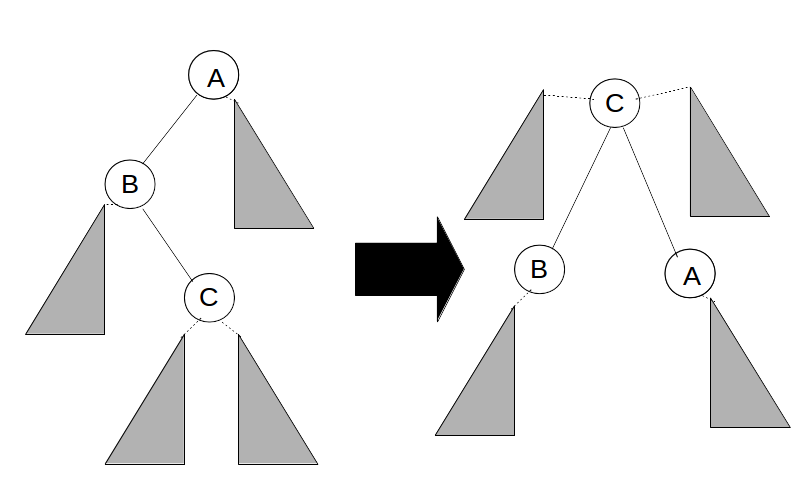
\includegraphics[scale=0.5]{Tango_path2.png}  

\subsection{Operacje na drzewie pomocniczym} Do zdefiniowania operacji słownikowych na drzewie Tango będziemy korzystali z następujących operacji na drzewie czerwono-czarnym. 
\begin{enumerate} 
\item{Split- Rozdzielenie drzewa czerwono-czarnego na dwa osobne zbilansowane drzewa, zawierające klucze mniejsze i większe od danego} 
\item{Join- Połączenie dwóch drzew czerwono-czarnych w jedno} 
\end{enumerate} 
\subsection{Łączenie i rozdzielanie drzew preferowanych ścieżek} 
Aby aktualizować preferowane ścieżki, potrzebujemy umieć połączyć dwa drzewa preferowanych ścieżek oraz rozdzielić drzewo preferowanej ścieżki. Do połączenia dwóch drzew wystarczy wykorzystać operację join. Aby rozdzielić ścieżkę w danym wierzchołku $w$, potrzebujemy znaleźć w drzewie pomocniczym wszystkie wierzchołki o głębokości większej niż \(\mathcal{D}(w)\) i zrobić z nich osobne drzewo pomocnicze. Zauważmy, że istnieje przedział kluczy, dla których wszystkie wierzchołki w drzewie pomocniczym są głębokości większej niż \(\mathcal{D}(w)\). Korzystając z maksymalnej głębokości, możemy znaleźć minimalny i maksymalny klucz o głębokości większej niż \(\mathcal{D}(w)\). Następnie przy pomocy dwóch operacji Split wydzielamy dolną część ścieżki do osobnego drzewa pomocniczego i łączymy z powrotem pozostałe klucze przy pomocy operacji join.\\ 
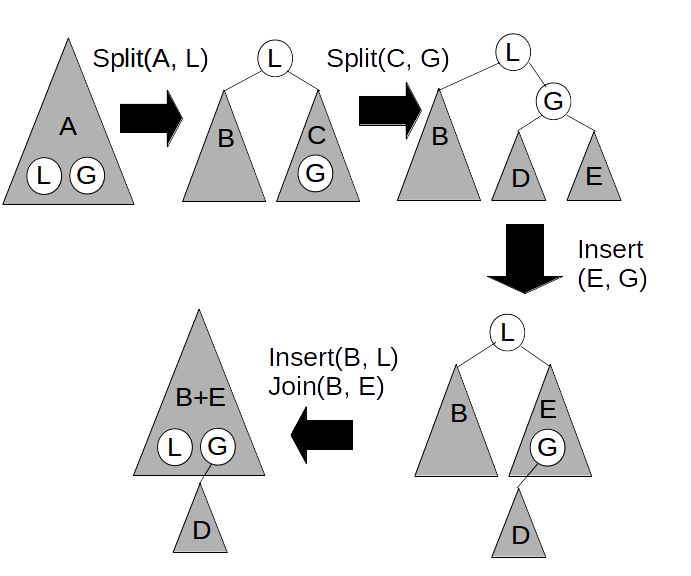
\includegraphics[scale=0.5]{rozdzielanie.png} 
\subsection{Aktualizacja preferowanych ścieżek} Mając wierzchołek $v$ chcemy zaktualizować drzewo w taki sposób, aby ścieżka do wierzchołka $v$ była ścieżką preferowaną całego drzewa. Niech wierzchołek $v$ będzie częścią preferowanej ścieżki \(\mathcal{P}\), jakiegoś poddrzewa drzewa referencyjnego. \(\mathcal{P}\) może być pojedynczym wierzchołkiem. Zaczynamy od rozdzielenia \(\mathcal{P}\) w wierzchołku $v$. Preferowany syn wierzchołka, jeżeli istnieje, staje się nie preferowanym synem. Następnie wykonujemy poniższe kroki, tak długo, aż nie dotrzemy do korzenia całego drzewa. 
\begin{enumerate} 
\item{Niech $v$ będzie ostatnim elementem preferowanej ścieżki z wierzchołka $r$. Znajdujemy ojca $o$ wierzchołka $r$.} 
\item{Rozdzielamy ścieżkę preferowaną do której należy $o$ w wierzchołku $o$. Preferowany syn wierzchołka staje się nie preferowanym.} 
\item{Do górnej części ścieżki preferowanej dołączamy ścieżkę z $r$ do $v$.} 
\end{enumerate} 
\subsection{Wyszukiwanie} Do wyszukiwania klucza $k$ będziemy symulować wyszukiwanie na drzewie referencyjnym. Najpierw wyszukujemy $k$ w drzewie pomocniczym. Jeśli nie znaleźliśmy klucza $k$ w ścieżce preferowanej, wtedy kontynuujemy wyszukiwanie w poddrzewie niepreferowanego syna ostatniego wierzchołka, na którym zakończyliśmy wyszukiwanie. Na koniec aktualizujemy preferowane ścieżki. 
\section{Analiza złożoności} 
\subsection{Złożoność czasowa} Oszacujmy złożoność operacji na drzewach pomocniczych. 
\begin{lemma} 
\label{Pref_cost} 
Złożoność dowolnej operacji na drzewie pomocniczym to \( O(\log \log n)\) gdzie $n$ to liczba elementów w strukturze. 
\end{lemma} 
\begin{proof} 
Preferowane ścieżki, są ścieżkami zbilansowanego drzewa binarnego, zatem ich długość jest nie większa niż \(\lceil \log n \rceil\). Operacje na drzewach pomocniczych są implementowane przy pomocy drzewa czerwono-czarnego i są wykonywane w czasie logarytmicznym od rozmiaru drzewa. Zatem koszt operacji to \( O(\log\log n)\). 
\end{proof}  

Następnie oszacujmy koszt pojedynczego dostępu do elementu w drzewie Tango.
\begin{lemma} 
\label{Tango_cost} Złożoność pojedynczego dostępu do elementu \(x_i\) w drzewie Tango to \(O((k+1)(1+loglogn))\), gdzie $n$ to liczba elementów w strukturze, a $k$ liczba nie preferowanych krawędzi na ścieżce z korzenia do \(x_i\). 
\end{lemma} 
\begin{proof} Koszt dostępu można rozdzielić na koszt wyszukiwania i koszt aktualizacji preferowanych ścieżek w drzewie. Przy wyszukiwaniu odwiedzimy nie więcej niż $k+1$ drzew pomocniczych. Z \ref{Pref_cost} wynika, że wyszukiwanie w drzewie pomocniczym ma złożoność \(O(loglogn)\). Zatem sumaryczny koszty wyszukania to \(O((k+1)(1+loglogn))\). Analogicznie przy aktualizacji dla każdego odwiedzonego drzewa pomocniczego wykonujemy jedna operację Split i dwie operacje Join, wiec sumaryczny koszt to również\(O((k+1)(1+loglogn))\). 
\end{proof} 
\begin{theorem} Pesymistyczny koszt pojedynczego dostępu to \(O(log(n)log(log(n)))\). 
\end{theorem} 

\subsection{Złożoność pamięciowa} Dla każdego wierzchołka będziemy pamiętać maksymalnie dwa wskaźniki na synów w drzewie pomocniczym, dwa wskaźniki na nie preferowanych synów w drzewie referencyjnym, jeden wskaźnik na ojca w drzewie pomocniczym, oraz klucz. Zatem złożoność pamięciowa to \( O (n)\). 

\section{Konkurencyjność}   

\subsection{Przeplotowe ograniczenie dolne} Zdefiniujemy sobie model do szacowania ograniczenia dolnego na liczbę operacji na optymalnym drzewie binarnym. Stwórzmy na kluczach $x_i \in \{1, ..., n\}$ idealne drzewo binarne \(B\). Jeśli \( n \neq 2^k -1\) wtedy nasze drzewo będzie pełne, a nie idealne. Struktura drzewa nie będzie się zmieniać w czasie.  

\begin{definition}[Lewy i prawy obszar] 
Dla danego wierzchołka \(y\) i drzewa \(B\) jego lewym obszarem \(L(y)\) będzie lewe poddrzewo \(y\) oraz \(y\), a prawy obszar \(P(y)\) to prawe poddrzewo \(y\).
\end{definition}  

Przy każdym zapytaniu \(x_i\) dla wszystkich wierzchołków na ścieżce od korzenia do \(x_i\) odnotowujemy czy \(x_i\) znajduje się w jego prawym czy lewym poddrzewie.  

\begin{definition}[Przeplot] 
Dla danego wierzchołka \(y\), drzewa \(B\) i ciągu zapytań \(X\), przeplotem nazwiemy parę zapytań \((x_i, x_j)\) spełniającą następujące warunki : \\ 
\begin{enumerate} 
\item{\( ( x_i \in P(y) \wedge x_j \in L(y)) \vee ( x_i \in L(y) \wedge x_j \in P(y))\)} 
\item{\( \neg \exists_{k \in [i, j]}( x_k \in  L(y) \vee x_k \in P(y) \)} 
\end{enumerate}  

Zdefiniujmy, także funkcję \(IB(X, i)\) jako liczbę przeplotów wprowadzonych przez i-te zapytanie, w ciągu zapytań $X$, a \(IB(X) = \sum_i IB(X, i)\). \end{definition}  

Będziemy starali oszacować liczbę operacji w optymalnym algorytmie BST, korzystając z liczby przeplotów. Niech \(T_i\) będzie stanem drzewa binarnego po wykonaniu zapytań \( x_1, x_2, ..., x_i\), przez dowolny deterministyczny algorytm wyszukiwania i reorganizacji.  

\begin{definition} Punkt przejściowy wierzchołka $y$ w momencie $i$ to wierzchołek $z$ , o najmniejszej  głębokości w \( T_i\), taki że ścieżka z korzenia $T_i$ przechodzi przez jakiś wierzchołek zarówno z $L(y)$ jaki i $P(y)$ w pełnym drzewie $B$. \end{definition}  

\begin{lemma} 
Dla każdego wierzchołka $y$ i momentu $i$ istnieje dokładnie jeden punkt przejściowy. 
\end{lemma} 
\begin{proof} 
Niech $l$ i $r$ będą najniższymi wspólnymi przodkami odpowiednio wierzchołków z $L(y)$ i  z $P(y)$ w $T_i$ . Ponieważ klucze w lewym obszarze stanowią spójny przedział posortowanego ciągu wszystkich kluczy, a w drzewie BST wspólny przodek dwóch wierzchołków ma wartość klucza pomiędzy wartościami synów, w takim razie $l$ jest elementem lewego poddrzewa. Analogicznie $r$ jest elementem prawego poddrzewa. Zauważmy również, że klucze całego poddrzewa $y$ w $B$ stanowią spójny przedział posortowanego ciągu wszystkich kluczy, zatem najniższy wspólny przodek należy albo do lewego albo do prawego obszaru. Z tego wynika, że $l$ lub $r$ jest najniższym wspólnym przodkiem całego poddrzewa. Załóżmy bez straty ogólności, że jest to $l$. Zauważmy, że $r$ będzie punktem przejściowym dla $y$ w momencie $i$. Z definicji, najniższego wspólnego przodka, jest jedynym wierzchołkiem o najmniejszej głębokości, którego ścieżka przechodzi przez wierzchołek z $R(y)$. Ścieżka do $r$ przechodzi też przez $l$, które jest elementem $L(y)$. \end{proof}  

\begin{lemma} 
Jeśli w momencie $i$ $z$ był punktem przejściowym wierzchołka $y$ i algorytm BST obsługując zapytania $x_j, ..., x_k$  nie przechodzi przez $z$, ani nie wykonuje rotacji, która by zmniejszyła głębokość $z$, to $z$ jest punktem przejściowym w każdym momencie z przedziału \([j, k]\). 
\end{lemma}
\begin{proof} Zdefiniujmy $l$ i $r$ jak w poprzednim dowodzie i załóżmy bez straty ogólności, że $l$ jest wspólnym przodkiem wszystkich wierzchołków z $L(y)$ i $P(y)$ w momencie $j$. Zatem $r$ jest punktem przejściowym $y$ w momencie $j$. Skoro algorytm BST nie przechodzi w zapytaniach przez $r$ to $r$ pozostaje najniższym wspólnym przodkiem wierzchołków $P(Y)$ w $T_i$. Dodatkowo, skoro nie została wykonana, żadna rotacja zmniejszająca  głębokość $r$ to poddrzewo $r$ w \(T_i\) pozostaje niezmienne. W czasie wykonywania zapytań \( x_j,..., x_k\) , żaden element z $L(y)$ nie stał się synem $r$, zatem jakiś element $L(Y)$ musi być wspólnym przodkiem wszystkich wierzchołków z $L(y)$ i $P(y)$. Z tego wynika, że $r$ pozostaje punktem przejściowym $y$. 
\end{proof}  

\begin{lemma} 
\label{eig_trans_point} 
Każdy wierzchołek $z$ może być w momencie $i$ punktem przejściowym co najwyżej jednego wierzchołka $y$. 
\end{lemma} 
\begin{proof} 
Weźmy dowolne dwa wierzchołki $y_1$ i $y_2$, pokażemy, że ich punkty przejściowe w momencie $i$ są różne. Zdefiniujmy dla nich podobnie jak w dowodach poprzednich lematów odpowiednio $l_1, r_1$ i $l_2, r_2$. Jeśli $y_1$ i $y_2$ nie znajdują się na jednej ścieżce do korzenia ( żaden nie jest przodkiem drugiego), to ich lewe i prawe obszary są rozłączne, a zatem ich punkty przejściowe muszą być różne. Jeśli tak nie jest to załóżmy bez straty ogólności, że $y_1$, jest przodkiem $y_2$. Jeśli punkt przejściowy $y_1$ znajduje się w innym obszarze $y_1$ niż $y_2$, wtedy punkty przejściowe muszą być różne. W przeciwnym wypadku punkt przejściowy $y_1$ musi być wspólnym przodkiem elementów z $L(y_2)$ i $R(y_2)$. Zatem głębokość punktu przejściowego $y_1$ będzie nie większa niż głębokość $l_2$ i $r_2$. Z kolei punkt przejściowy $y_2$ ma głębokość nie mniejszą niż głębokości $l_2$ i $r_2$. Skoro $l_2$ i $r_2$ muszą mieć różne głębokości, to punkty przejściowe $y_1$ i $y_2$ muszą być różne.  
\end{proof} 
\begin{theorem} 
\label{low_bound} 
\(OPT(X) \geq \frac{IB(X)}{2} - n\), gdzie $OPT$ to koszt działania optymalnego algorytmu BST na ciagu zapytań $X$. 
\end{theorem} 
\begin{proof} 
Będziemy szacować z dołu liczbę operacji wykonywanych przez optymalny algorytm przez liczbę punktów przejściowych odwiedzonych (przechodzi przez nie ścieżka z korzenia do $x_i$ lub wykonuje się na nich rotacje zmniejszające ich głębokość) w trakcie wykonywania zapytań. Korzystając z \ref{eig_trans_point} będziemy zliczać te wydarzenia dla każdego wierzchołka $y$ osobno, a następnie je zsumujemy. Niech \( x_{a_1}, x{a_2}, ..., x{a_k}\) będzie maksymalnym podciągiem zapytań, w którym każde dwa kolejne zapytania są o elementy w różnych obszarach $y$. $p$ będzie liczbą przeplotów w $y$. Załóżmy bez straty ogólności, że zapytania \(x_{a_{2i}}\) będą zapytaniami a elementy lewego obszary, \(x_{a_{2i+1}}\) prawego. Rozpatrzmy $l$ i $r$ takie jak w poprzednich dowodach. Wszystkie zapytania o prawy obszar $y$ odwiedzają $r$, a o lewy odwiedzają $l$. Zatem przy dwóch kolejnych zapytaniach albo algorytm albo będzie przechodził przez punkt przejściowy przy wyszukiwaniu, albo punkt przejściowy się zmieni, co również wymaga odwiedzenia punktu przejściowego. Zatem dla dwóch kolejnych zapytań z naszego podciągu algorytm przynajmniej raz odwiedza punkt przejściowy $y$. Dla danego wierzchołla otrzymujemy odwiedzamy \(\lfloor \frac{p}{2} \rfloor \geq \frac{p}{2} -1\).  Sumując po wszystkich $y$ otrzymujemy \(OPT(X) \geq \frac{IB(X)}{2} - n\). 
\end{proof}  


\subsection{Zastosowanie przeplotów w oszacowaniu konkurencyjności} 
\begin{lemma}
\label{num_switch} 
Liczba nie preferowanych krawędzi na ścieżce z korzenia do \(x_i\) jest równa \(IB(X, i)\). 
\end{lemma} 
\begin{proof} 
Obecność niepreferowanej krawędzi \( \{a, b\}\) na ścieżce oznacza, że ostatnie zapytanie o element w poddrzewie wierzchołka $y$ w innym poddrzewie niż \(x_i\). To odpowiada przeplotowi. 
\end{proof}  

\begin{theorem} 
Dla ciągu zapytań \(X = \{x_1, x_2,..., x_m\}\), takich że \( \forall_i x_i \in \{1, 2, ..., n\}\) sumaryczny koszt działania drzewa Tango to \( O((OPT(X) + n)(1 + loglogn))\), gdzie \(OPT(X)\) to koszt optymalnego dynamicznego drzewa BST działającego offline. 
\end{theorem} 
\begin{proof} 
Z \ref{num_switch} i \ref{Tango_cost} wynika, że koszt obsługi pojedynczego zapytania na drzewie Tango to \(O((IB(X, i)+1)(1+loglogn))\).Dodatkowo, dla każdego wierzchołka co najwyżej raz będziemy zmieniać jego stan z nie posiadania preferowanego syna na posiadanie jednego. Zatem sumaryczny koszt zapytania to \(O((IB(X)+m +n )(1+loglogn))\). Z \ref{low_bound} wiemy, że \(OPT(X) \geq IB(X) - n\). Oczywiste też jest, że \(OPT(X) \geq m\). Z tego wynika, że koszt algorytmu to \(O(OPT(X)+n )(1+loglogn))\). 
\end{proof}  

\section{Opis implementacji} 

Implementacja składa się z dwóch klas \texttt{br\_tree},\texttt{br\_vert}\texttt{tango\_tree} i\texttt{tango\_vert}. 

\subsection{br\_vert}

Ta klasa reprezentuje wierzchołek drzewa czerwono-czarnego oraz jego poddrzewo. Ta klasa dziedziczy po wcześniej wymienionej klasie \texttt{tree\_vert}. Rozszerza funkcjonalność klasy bazowej o aktualizowanie czarnej wysokości przy zmianach w strukturze drzewa oraz o następujące metody

\begin{itemize}

\item{Konstruktor \texttt{tree\_vert(T val, tree\_vert<T>*f = NULL, tree\_vert<T>*l = NULL, tree\_vert<T>*r = NULL, bool is\_null = false)} tworzący wierzchołek trzymający wartość. Umożliwia ustawienie ojca wierzchołka (f), lewego syna (l), prawego syna (r) oraz wartość oznaczającą czy wartość w wierzchołku ma być traktowana jako cześć drzewa (is\_null)}

\item{\texttt{ br\_vert<T>* parent(), br\_vert<T>* left\_son(), br\_vert<T>* right\_son(), br\_vert<T>* grandparent(),br\_vert<T>* uncle(),br\_vert<T>* brother()} - zwracają }
    
\item{\texttt{bool hook\_up\_left(tree\_vert<T>*)} i \texttt{bool hook\_up\_right(tree\_vert<T>*)} - podpinają wierzchołek z argumentu jako odpowiednio lewego i prawego syna wierzchołka.}

\item{\texttt{bool get\_disowned()} - rozcina krawędź pomiędzy wierzchołkiem a jego ojcem}

\item{\texttt{bool is\_root(), bool is\_left(),  bool is\_right()} - sprawdzają czy wierzchołek jest korzeniem, lewym synem czy prawym synem}

\item{\texttt{void rotate\_left(), void rotate\_right()} - wykonują rotację ojca wierzchołka}
    
\item{\texttt{void splay()} - wykonuje operację splay na danym wierzchołku}
    
\item{\texttt{tree\_vert<T>* search( T )} - wyszukuje klucza danego jako argument w poddrzewie wierzchołka i zwraca ostatni napotkany wierzchołek}
   
\item{\texttt{tree\_vert<T>* next() ,  tree\_vert<T>* prev()} - zwracają natępnika oraz poprzednika wierzchołka w drzewie}
\end{itemize}

\section{br\_tree}

Ta klasa reprezentuje całe drzewo splay. Udostępnia następujące metody: 

\begin{itemize}

\item{Konstruktory \texttt{splay\_tree(),splay\_tree(tree\_vert<T>*) } tworzące puste drzewo i drzewo danym korzeniu }

\item{Desktruktor zwalniający wszystkie wskaźniki w drzewie}

\item{\texttt{void splay(T)} - wykonuje operację splay na ostatnim wierzchołku na ścieżce wyszukiwania klucza podanego jako argument}

\item{\texttt{bool find(T)} - sprawdza czy element znajduje się w drzewie}
    
\item{\texttt{tree\_vert<T>* lower\_bound( T ), tree\_vert<T>* upper\_bound( T ) } - wyszukują klucza danego jako argument w drzewie i zwraca wskażniki na odpowiednio najmniejszy element większy równy i najmniejszy element mniejszy równy. Gdy wynik nie istnieje zwraca NULL }
   
\item{\texttt{bool insert(T)} - wstawia element do drzewa zwraca \texttt{false} jeśli element znajdował sie wcześniej w drzewie oraz \texttt{true} w przeciwnym wypadku}
\item{\texttt{bool erase(T)} - wstawia element do drzewa zwraca \texttt{true} jeśli element znajdował sie wcześniej w drzewie oraz \texttt{false} w przeciwnym wypadku}

\end{itemize}

Dodatkowo na drzewach splay są dostępne następujące funkcje : 

\begin{itemize}

\item{\texttt{vector<splay\_tree<T>* > split(splay\_tree<T>* tree, T searched)} - rozdziela drzewo tree na drzewa z elementami mniejszymi, równymi i większymi od podanej wartości}
\item{\texttt{splay\_tree<T>* join( splay\_tree<T>* lesser, splay\_tree<T>* greater)} - wykonuje operację join na dwóch drzewach}

\end{itemize}


\subsection{br\_vert}

Ta klasa reprezentuje wierzchołek drzewa czerwono-czarnego oraz jego poddrzewo. Ta klasa dziedziczy po wcześniej wymienionej klasie \texttt{tree\_vert}. Rozszerza funkcjonalność klasy bazowej o aktualizowanie czarnej wysokości przy zmianach w strukturze drzewa oraz o następujące metody

\begin{itemize}

\item{Konstruktor \texttt{tree\_vert(T val, tree\_vert<T>*f = NULL, tree\_vert<T>*l = NULL, tree\_vert<T>*r = NULL, bool is\_null = false)} tworzący wierzchołek trzymający wartość. Umożliwia ustawienie ojca wierzchołka (f), lewego syna (l), prawego syna (r) oraz wartość oznaczającą czy wartość w wierzchołku ma być traktowana jako cześć drzewa (is\_null)}

\item{\texttt{ br\_vert<T>* parent(), br\_vert<T>* left\_son(), br\_vert<T>* right\_son(), br\_vert<T>* grandparent(),br\_vert<T>* uncle(),br\_vert<T>* brother()} - zwracają }
    
\item{\texttt{bool hook\_up\_left(tree\_vert<T>*)} i \texttt{bool hook\_up\_right(tree\_vert<T>*)} - podpinają wierzchołek z argumentu jako odpowiednio lewego i prawego syna wierzchołka.}

\item{\texttt{bool get\_disowned()} - rozcina krawędź pomiędzy wierzchołkiem a jego ojcem}

\item{\texttt{bool is\_root(), bool is\_left(),  bool is\_right()} - sprawdzają czy wierzchołek jest korzeniem, lewym synem czy prawym synem}

\item{\texttt{void rotate\_left(), void rotate\_right()} - wykonują rotację ojca wierzchołka}
    
\item{\texttt{void splay()} - wykonuje operację splay na danym wierzchołku}
    
\item{\texttt{tree\_vert<T>* search( T )} - wyszukuje klucza danego jako argument w poddrzewie wierzchołka i zwraca ostatni napotkany wierzchołek}
   
\item{\texttt{tree\_vert<T>* next() ,  tree\_vert<T>* prev()} - zwracają natępnika oraz poprzednika wierzchołka w drzewie}
\end{itemize}

\section{br\_tree}

Ta klasa reprezentuje całe drzewo splay. Udostępnia następujące metody: 

\begin{itemize}

\item{Konstruktory \texttt{splay\_tree(),splay\_tree(tree\_vert<T>*) } tworzące puste drzewo i drzewo danym korzeniu }

\item{Desktruktor zwalniający wszystkie wskaźniki w drzewie}

\item{\texttt{void splay(T)} - wykonuje operację splay na ostatnim wierzchołku na ścieżce wyszukiwania klucza podanego jako argument}

\item{\texttt{bool find(T)} - sprawdza czy element znajduje się w drzewie}
    
\item{\texttt{tree\_vert<T>* lower\_bound( T ), tree\_vert<T>* upper\_bound( T ) } - wyszukują klucza danego jako argument w drzewie i zwraca wskażniki na odpowiednio najmniejszy element większy równy i najmniejszy element mniejszy równy. Gdy wynik nie istnieje zwraca NULL }
   
\item{\texttt{bool insert(T)} - wstawia element do drzewa zwraca \texttt{false} jeśli element znajdował sie wcześniej w drzewie oraz \texttt{true} w przeciwnym wypadku}
\item{\texttt{bool erase(T)} - wstawia element do drzewa zwraca \texttt{true} jeśli element znajdował sie wcześniej w drzewie oraz \texttt{false} w przeciwnym wypadku}

\end{itemize}

Dodatkowo na drzewach splay są dostępne następujące funkcje : 

\begin{itemize}

\item{\texttt{vector<splay\_tree<T>* > split(splay\_tree<T>* tree, T searched)} - rozdziela drzewo tree na drzewa z elementami mniejszymi, równymi i większymi od podanej wartości}
\item{\texttt{splay\_tree<T>* join( splay\_tree<T>* lesser, splay\_tree<T>* greater)} - wykonuje operację join na dwóch drzewach}

\end{itemize}


\chapter{Badanie wydajności drzew}
\section{Generowanie danych}
W niżej wymienionych eksperymentach drzewa są testowane na danych losowych typu \texttt{int} generowanych w następującje sposoby : 
\begin{itemize}
\item{Z rozkładem jednostajnym korzystając ze funkcji \texttt{uniform\_int\_distribution} ze standardowej biblioteki \texttt{random}.}
\item{Z rozkładem zbliżonym do rozkładu normalnego nakładając podłogę na wynik funkcji \texttt{normal\_distribution} i powtarzając losowania jeśli wynik wychodzi poza porządany przedział}
\item{Symulując przechodzenie po losowym drzewie nieskierowanym. Generuję losowe drzewo przy pomocy kodów Prüfera i kolejne zapytania odpowiadają kolejnym wierzchołkom na losowej ścieżce (nie musi być do ścieżka właściwa).}
\end{itemize}

\section{Testowanie dla problemu dynamicznej optymalności}
Zbadamy w jakim czasie obsługują zapytania implementacji poszczególnych struktur. Porównuję czasu działania drzew: Tango, Splay, czerwono-czarnego, statycznego drzewa optymalnego oraz standardowej struktury set. W tym eksperymencie nie bierzemy pod uwagę czasu budowania struktury. Wszystkie struktury zawierają elementy \(e_i \in [1, ..., n]\). Do struktury, do których elementy dodaje sie pojedynczo, czyli drzewa Tango, drzewa Splay oraz set, wstawiałam elementy w kolejności losowej (takiej samej dla wszystkich struktur). Zapytania są losowane przy pomocy wyżej wymienionych metod, tak aby \(\forall_i x_i \in [1, ..., n]\). Eksperyment powtarzam dla rosnących geometrycznie danych \( n = \{16, 32, 64, ..., 1024\}\). 

%%%%% BIBLIOGRAFIA

%\bibliographystyle{apacite}

\begin{thebibliography}{references}



\end{thebibliography}

\end{document}